\documentclass[aspectratio=169]{beamer}
\makeatletter
\def\input@path{{../common/}{../guide/}{../data/}{../code/}}
\makeatother
\usetheme{Bruno}
\usepackage{amsmath}
\usepackage{amssymb}
\usepackage{siunitx}
\usepackage{float}
\usepackage{tikz}
\def\checkmark{\tikz\fill[scale=0.4](0,.35) -- (.25,0) -- (1,.7) -- (.25,.15) -- cycle;} 
\usepackage{url}
\usepackage[siunitx,american,RPvoltages]{circuitikz}
\ctikzset{capacitors/scale=0.7}
\ctikzset{diodes/scale=0.7}
\usepackage{tabularx}
\newcolumntype{C}{>{\centering\arraybackslash}X}
\renewcommand\tabularxcolumn[1]{m{#1}}% for vertical centering text in X column
\usepackage{tabu}
\usepackage[spanish,es-tabla,activeacute]{babel}
\usepackage{babelbib}
\usepackage{booktabs}
\usepackage{pgfplots}
\usepackage{hyperref}
\hypersetup{colorlinks = true,
            linkcolor = black,
            urlcolor  = blue,
            citecolor = blue,
            anchorcolor = blue}
\usepgfplotslibrary{units, fillbetween} 
\pgfplotsset{compat=1.16}
\usepackage{bm}
\usetikzlibrary{arrows, arrows.meta, shapes, 3d, perspective, positioning,mindmap,trees,backgrounds}
\renewcommand{\sin}{\sen} %change from sin to sen
\usepackage{bohr}
\setbohr{distribution-method = quantum,insert-missing = true}
\usepackage{elements}
\usepackage{verbatim}
\usepackage[edges]{forest}
\usepackage{etoolbox}
\usepackage{schemata}
\usepackage{appendix}
\usepackage{listings}

\definecolor{color_mate}{RGB}{255,255,128}
\definecolor{color_plas}{RGB}{255,128,255}
\definecolor{color_text}{RGB}{128,255,255}
\definecolor{color_petr}{RGB}{255,192,192}
\definecolor{color_made}{RGB}{192,255,192}
\definecolor{color_meta}{RGB}{192,192,255}
\newcommand\diagram[2]{\schema{\schemabox{#1}}{\schemabox{#2}}}

\definecolor{codegreen}{rgb}{0,0.6,0}
\definecolor{codegray}{rgb}{0.5,0.5,0.5}
\definecolor{codepurple}{rgb}{0.58,0,0.82}
\definecolor{backcolour}{rgb}{0.95,0.95,0.92}

\lstdefinestyle{mystyle}{
    backgroundcolor=\color{backcolour},   
    commentstyle=\color{codegreen},
    keywordstyle=\color{magenta},
    numberstyle=\tiny\color{codegray},
    stringstyle=\color{codepurple},
    basicstyle=\ttfamily\footnotesize,
    breakatwhitespace=false,         
    breaklines=true,                 
    captionpos=b,                    
    keepspaces=true,                 
    numbers=left,                    
    numbersep=5pt,                  
    showspaces=false,                
    showstringspaces=false,
    showtabs=false,                  
    tabsize=2
}

\lstset{style=mystyle}
\usepackage{unicode-math}
\setsansfont{Fira Sans}
\setmainfont{Fira Sans}
\setmathfont{Fira Math}

\title{Transductores \\ \emph{ópticos}}
\author{
    Juan J. Rojas
}
\institute{Instituto Tecnológico de Costa Rica}
\date{\today}
\background{background.jpg}
\begin{document}
\sisetup{unit-math-rm=\mathrm,math-rm=\mathrm} % change sinitx font
\sisetup{output-decimal-marker = {,}}
\maketitle

% Transductores ópticos
% 4.1. Fotoconductores
% 4.2. Fotodiodos
% 4.3. Fototransistores
% 4.4. Fotovoltaicos
% 4.5. Piroeléctricos y termopilas para radiación térmica


\newcommand{\blackandwhite}{white} %change this at the end

\begin{frame}[t]{Unidades ópticas}
    \begin{itemize}
        \item Steradian [sr] = ángulo sólido 
        \item Candela [cd] [W/sr] = intensidad luminosa, potencia irradiada por unidad de ángulo sólido
        \item Lumen [cd\cdot sr] = flujo luminoso, potencia irradiada
        \item Lux [cd\cdot sr/m\textsuperscript{2}] = iluminancia, flujo luminoso por unidad de área
        \item Candela por metro cuadrado [cd/m\textsuperscript{2}] = luminancia, intensidad luminosa por unidad de área
    \end{itemize}
\end{frame}

\begin{frame}{Fotoconductores}
    \begin{columns}[T, onlytextwidth]
        \begin{column}{0.55\textwidth}
            \begin{itemize}
                \item Aa
            \end{itemize}
        \end{column}
        \begin{column}{0.45\textwidth}
        \centering
        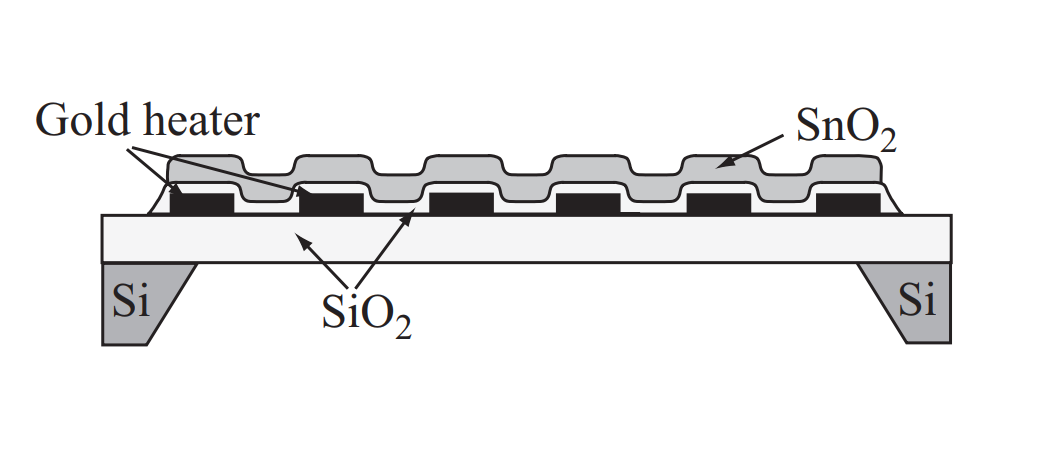
\includegraphics[width = \linewidth]{08_químicos/metal_oxido.png}
        \vspace*{1cm}
        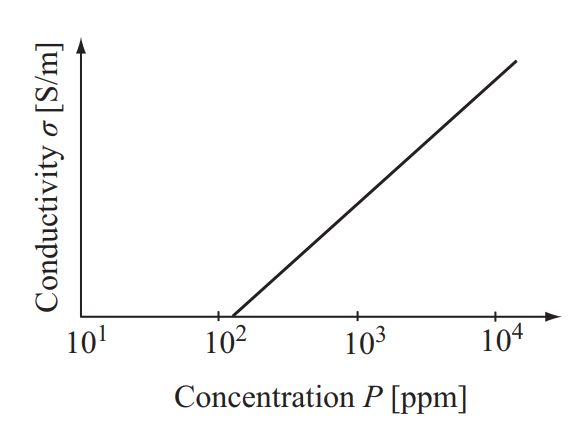
\includegraphics[width = 0.8\linewidth]{08_químicos/metal_oxido_sens.png}

        \tiny{Tomado de \cite{ida2013sensors}}
        \end{column}
    \end{columns}
\end{frame}

\begin{frame}{Referencias}
\footnotesize
\printbibliography[heading=none]
\end{frame}

\end{document}